\subsection{Aesthetic Prototype}
Our current prototype consists of two 3D-printed circular base plates sandwiching a 
75mm bar-type strain gauge load cell. Each plate is 110mm in diameter and 8mm thick, 
printed in PLA/PETG. The top plate has countersink pockets on the bottom face for M4 bolts 
that secure it to one end of the load cell, and the bottom plate attaches to the other end, sitting flat on the surface. The load cell wires route out to the HX711 amplifier and ESP32 on a nearby breadboard.

\subsubsection{Exploded View}
    Figure~\ref{fig:exploded} shows the exploded view of the load cell assembly with all components labeled.
    \begin{figure}[H]
    \centering
    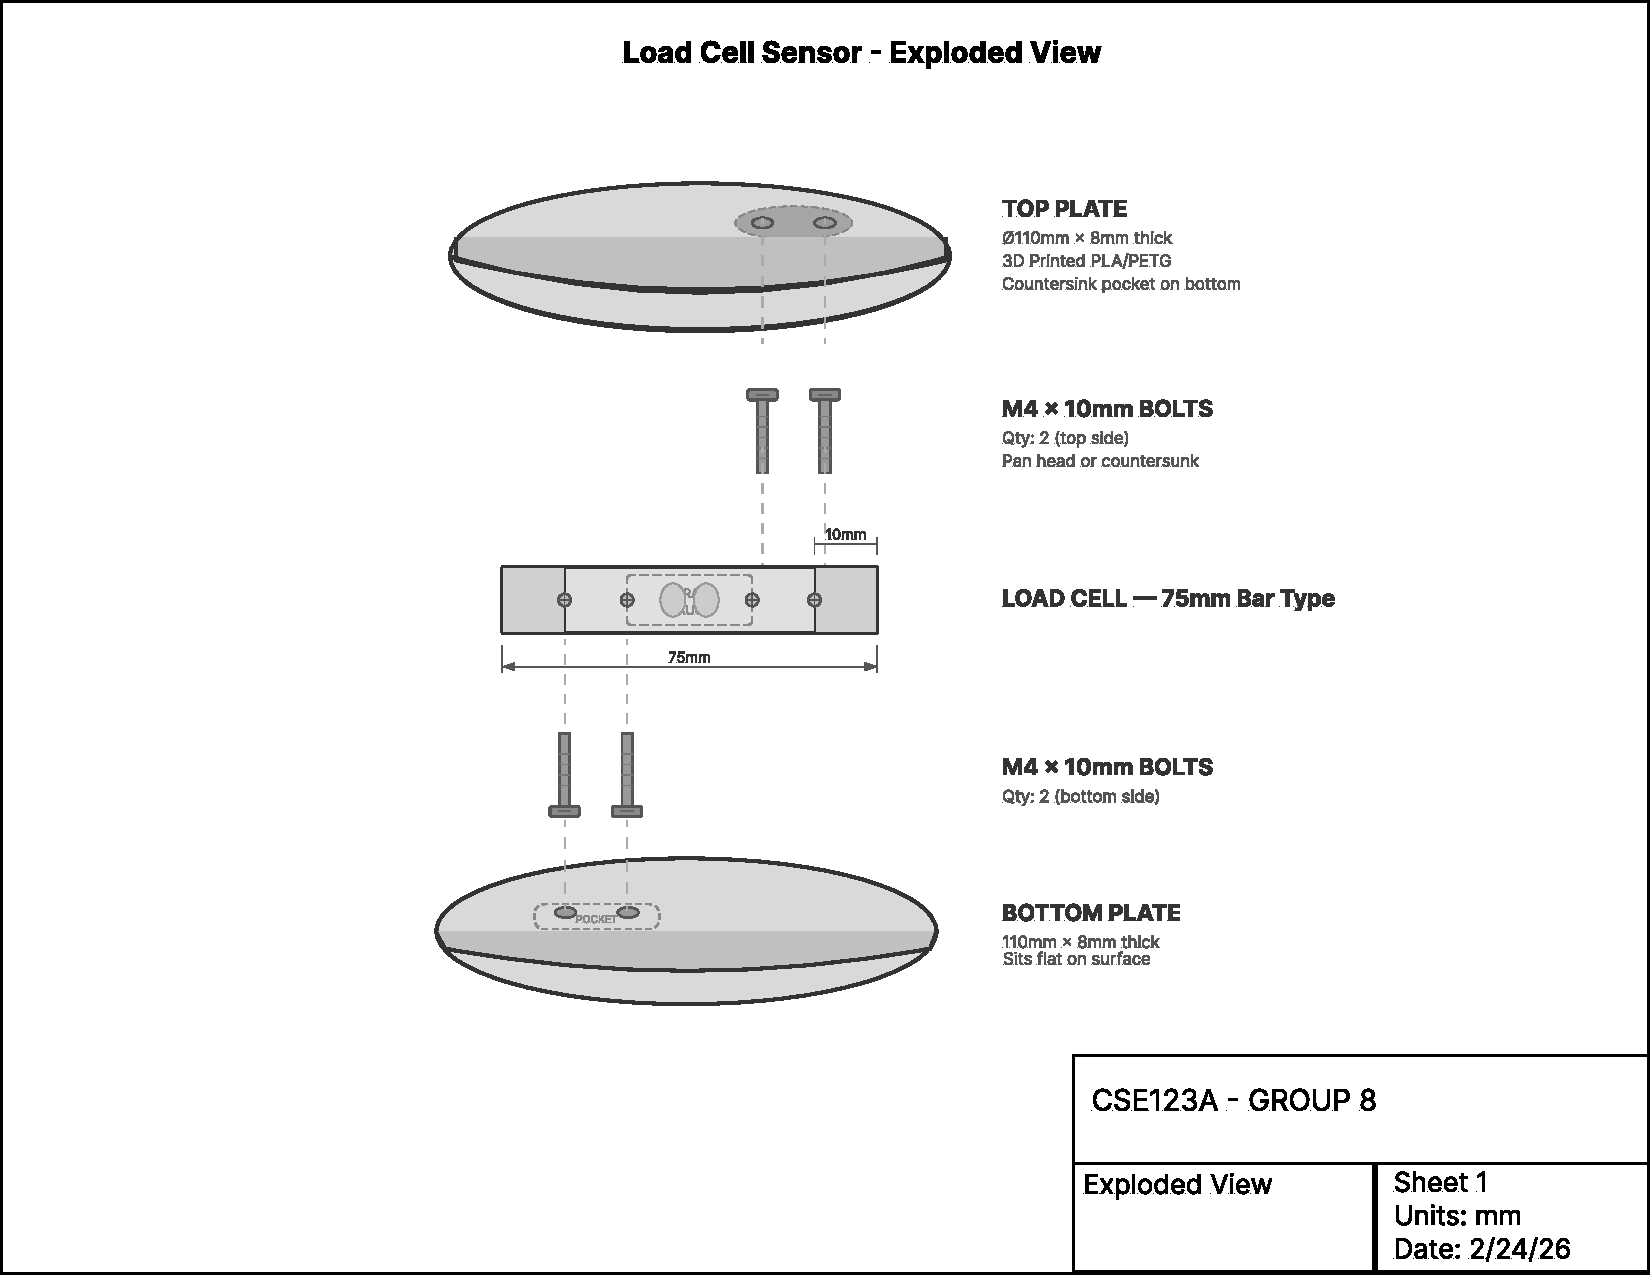
\includegraphics[width=0.7\textwidth]{../Documentation/Diagrams/Exploded-view.pdf}
    \caption{Exploded view of the load cell assembly showing top plate, bottom plate, load cell, and M4 hardware.}
    \label{fig:exploded}
    \end{figure}

\subsubsection{Base Plate Schematic}
    Figure~\ref{fig:schematic} shows the design schematic of the base plate with dimensions and screw hole placement.
    \begin{figure}[H]
    \centering
    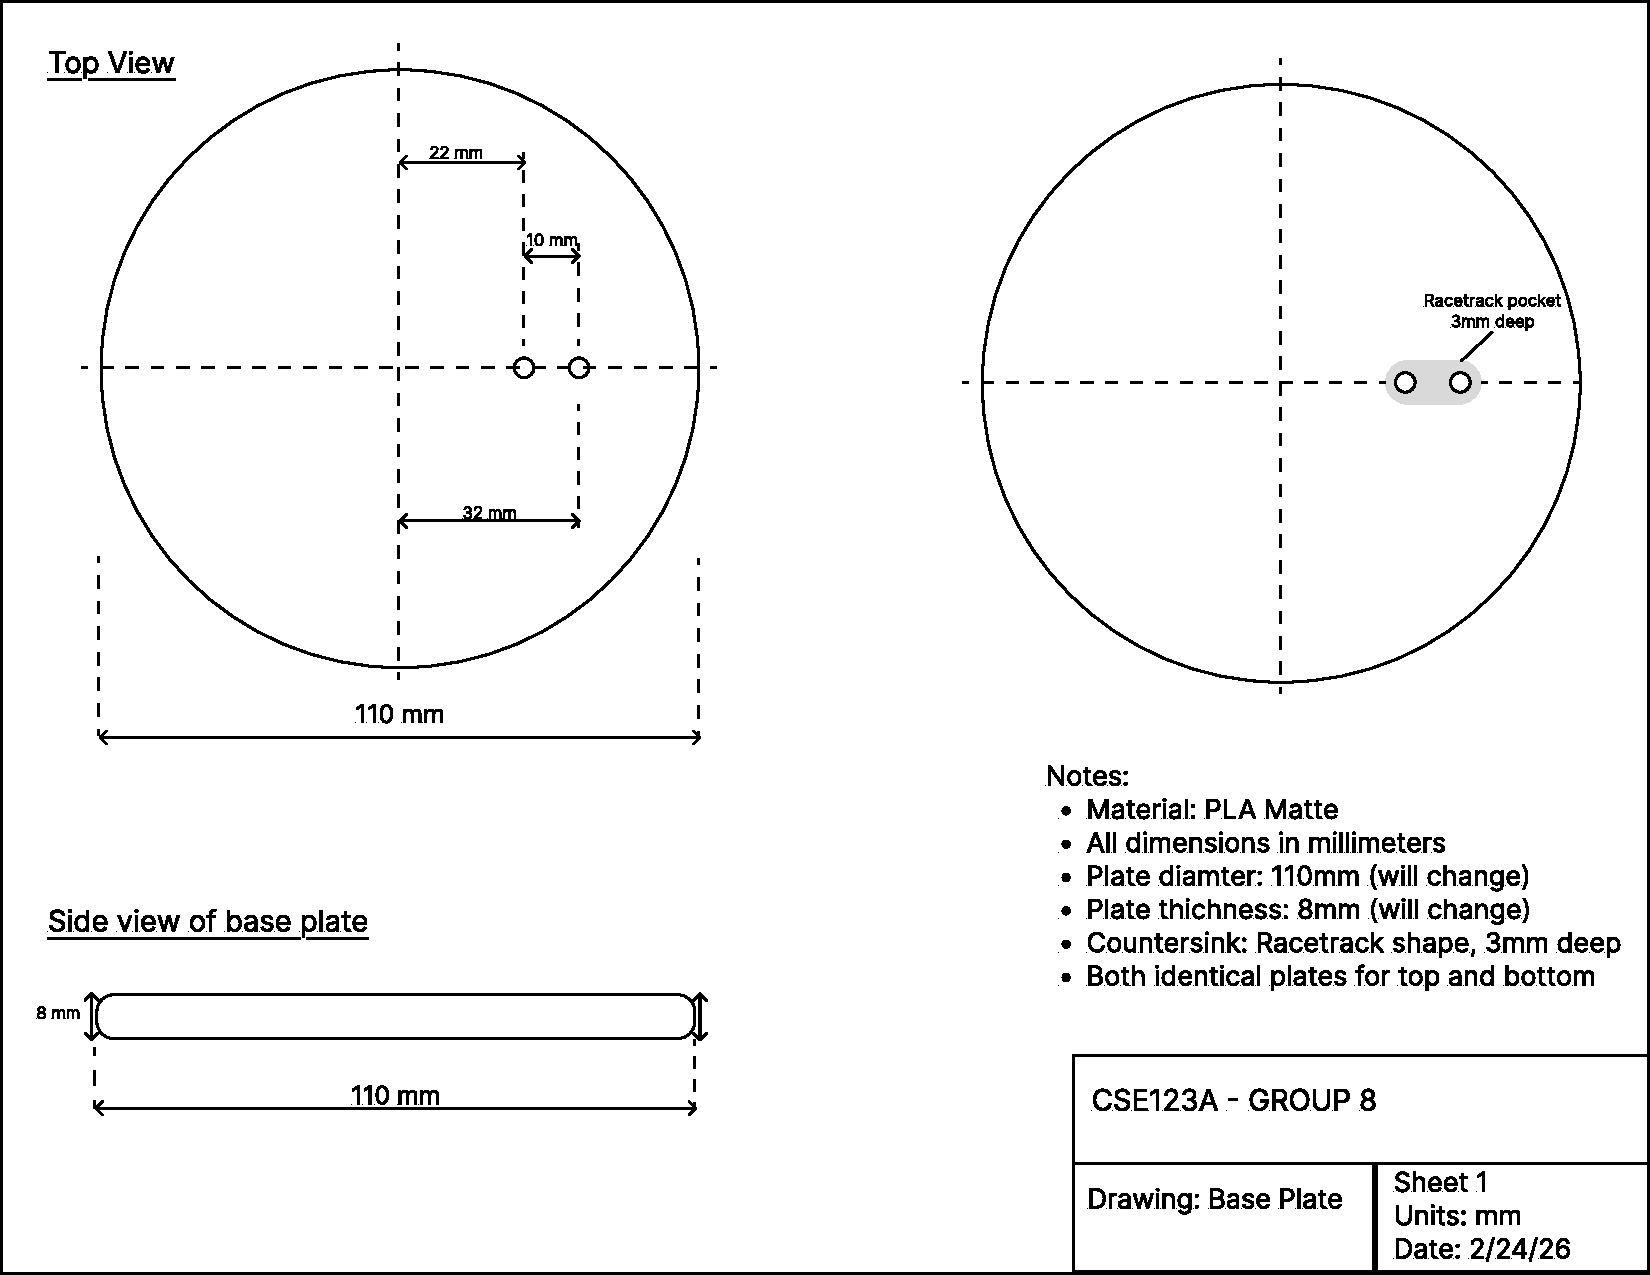
\includegraphics[width=0.7\textwidth]{../Documentation/Diagrams/Design-Schematic-of-baseplate-v2.pdf}
    \caption{Design schematic of the base plate.}
    \label{fig:schematic}
    \end{figure}

\subsubsection{Physical Prototype}
    Figure~\ref{fig:sideview} shows the assembled prototype from a side view, with the load cell mounted between the two plates and wired to the breadboard.
    \begin{figure}[H]
    \centering
    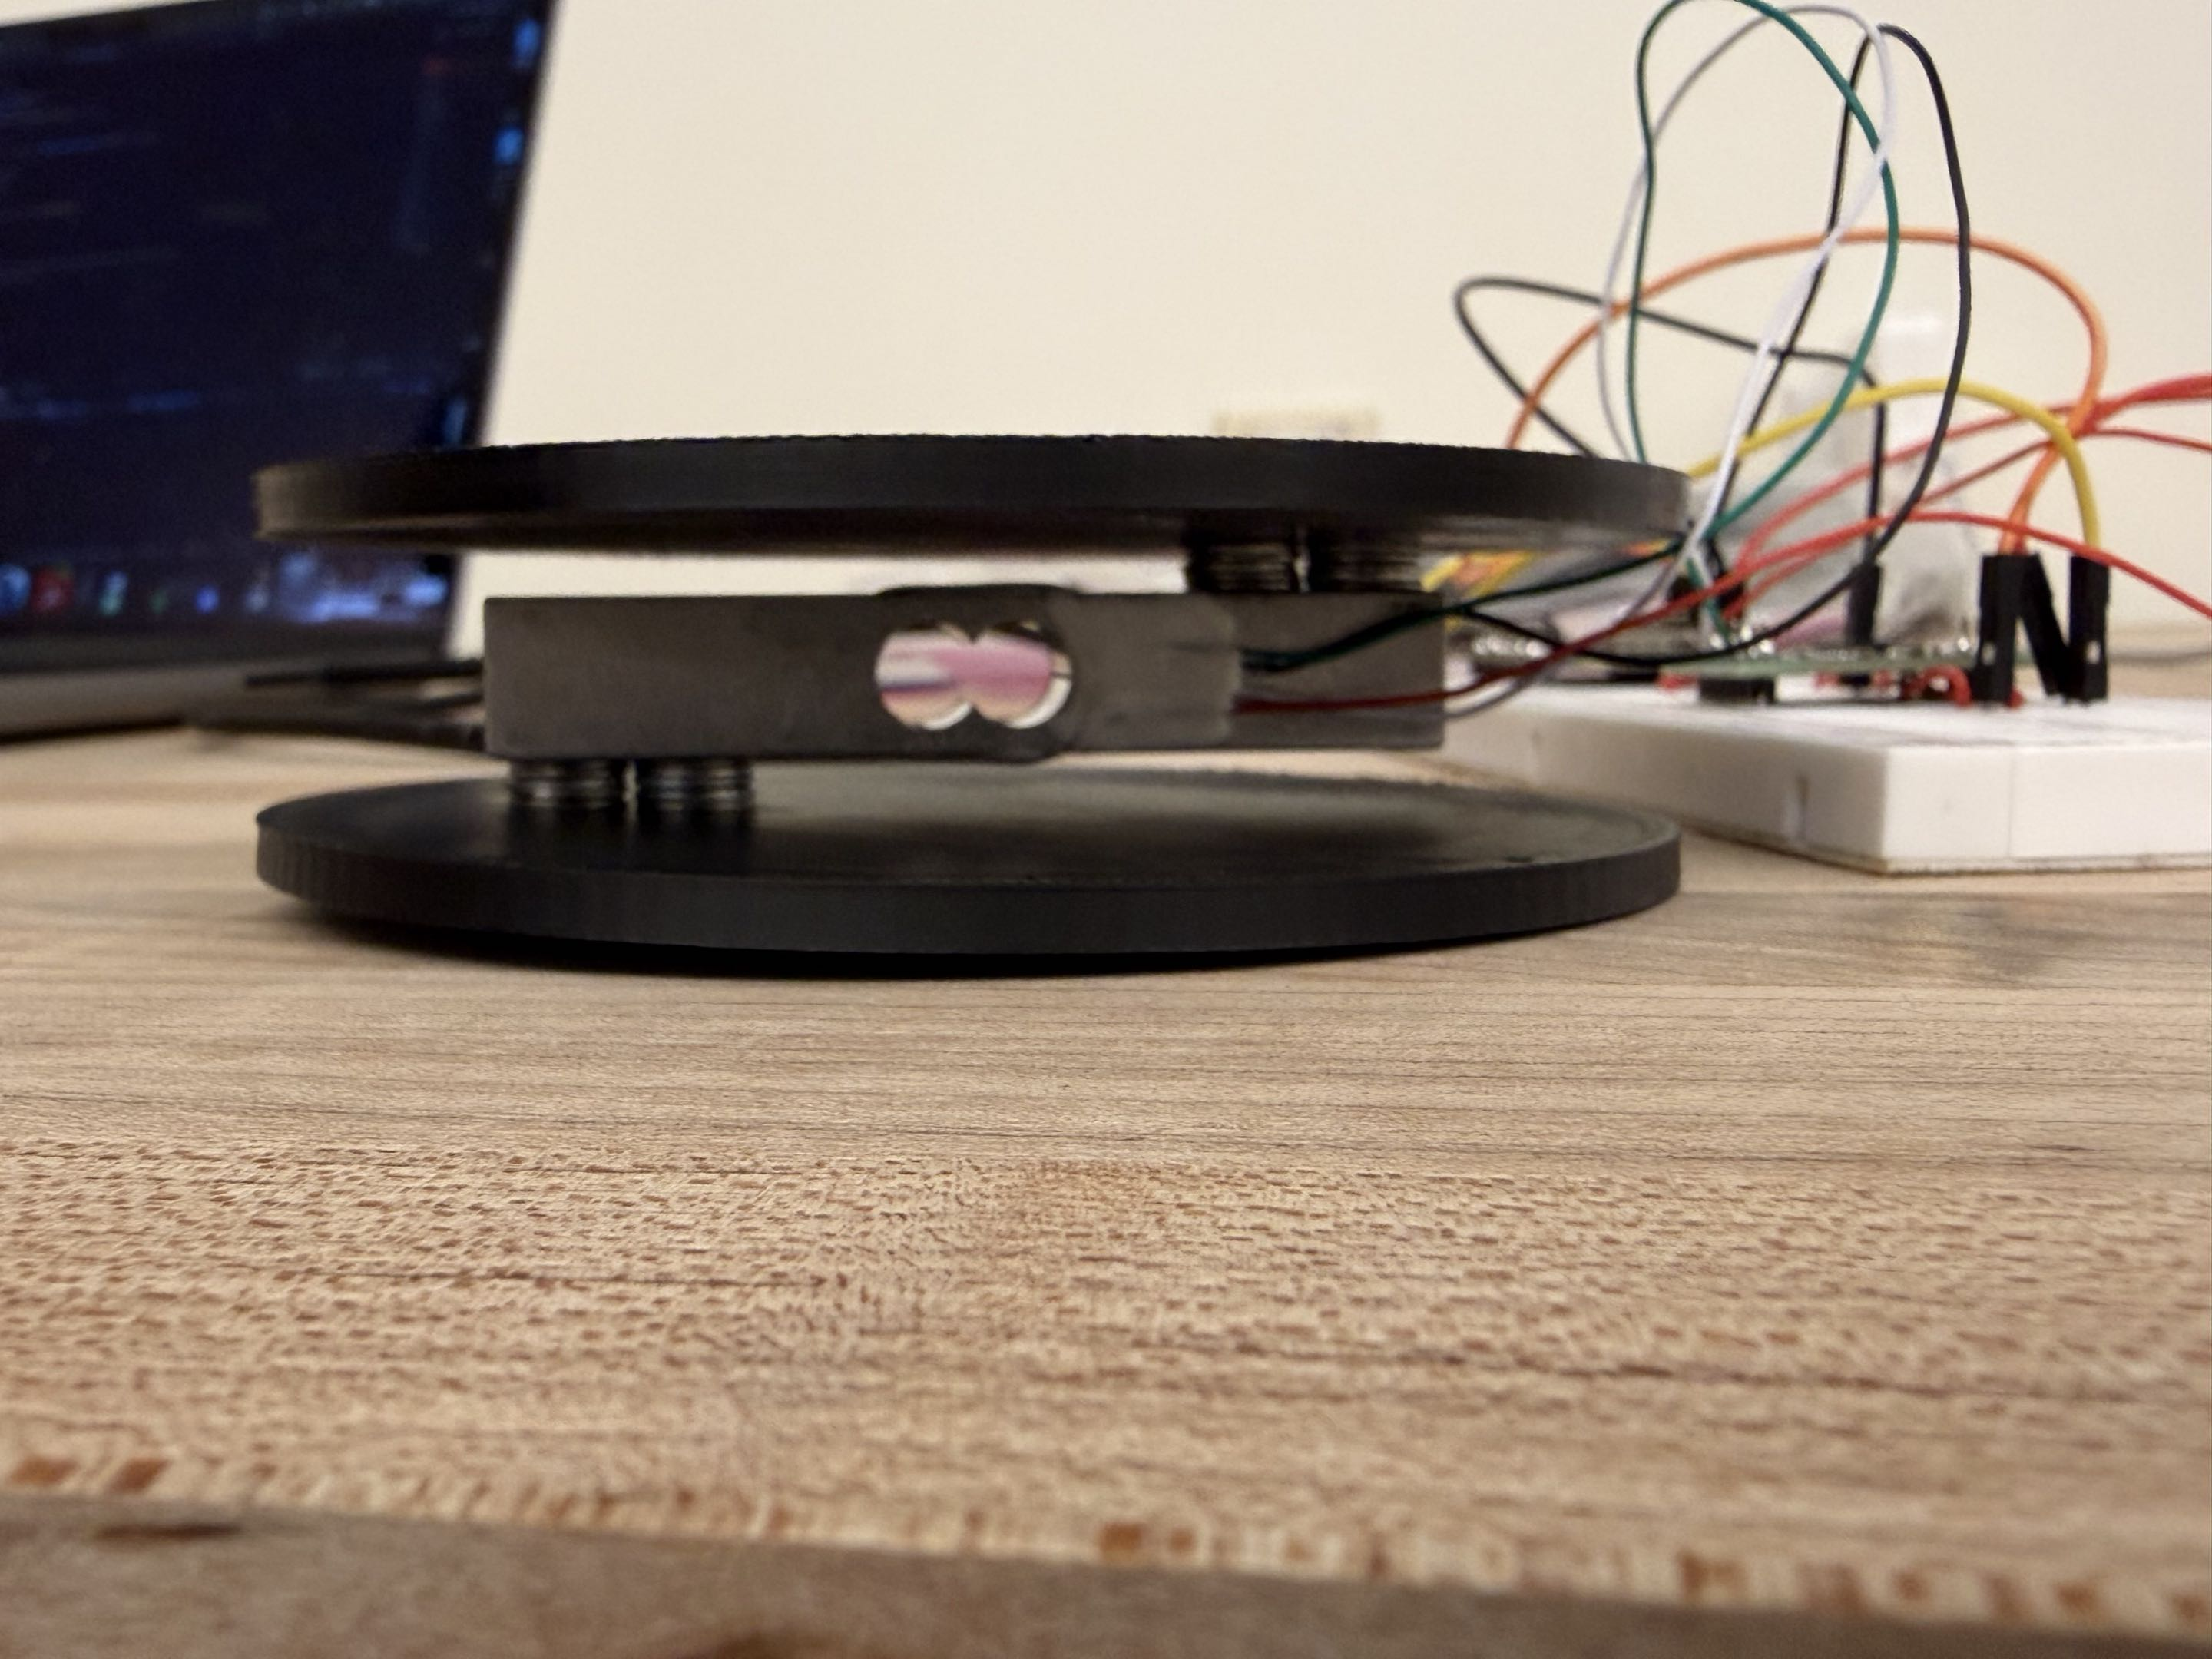
\includegraphics[width=0.5\textwidth]{../HardwarePicture/sideview.jpg}
    \caption{Side view of the assembled prototype showing the two base plates, load cell, and wiring to the ESP32.}
    \label{fig:sideview}
    \end{figure}
